\documentclass{standalone}
\usepackage{tikz}
\usepackage{ctex,siunitx,ninecolors}
\setCJKmainfont{Noto Serif CJK SC}
\usepackage{tkz-euclide}
\usepackage{amsmath}
\usepackage{wasysym}
\usetikzlibrary{patterns, calc}
\usetikzlibrary {decorations.pathmorphing, decorations.pathreplacing, decorations.shapes}
\newcommand{\posthead}[2][gray]{
  \begin{scope}[#2]
    \fill[left color=#1,right color= #1,middle color=#1!20](0,0)ellipse(0.05 and 0.02);
    \fill[left color=#1,right color= #1,middle color=#1!20](0.05,0)rectangle(-0.05,0.07);
    \fill[left color=#1,right color= #1,middle color=#1!20](-0.06,0.07)arc(-180:0:0.06 and 0.02)--(0.06,0.15)--(0.05,0.16)--(-0.05,0.16)--(-0.06,0.15)--cycle;
    \fill[#1!50!gray](0,0.16)ellipse(0.05 and 0.02);
    \foreach \x in {75,45,15,-15,-45,-75}
    {
      \draw[very thin,#1!50!gray]({0.05*sin(\x)},{0.16-0.02*cos(\x)})--({0.06*sin(\x)},{0.15-0.02*cos(\x)})--++(0,-0.08);
    }
  \end{scope}
}
\begin{document}
\small
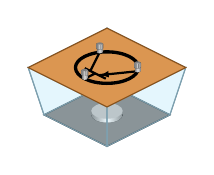
\begin{tikzpicture}[>=latex,scale=1.0]
  \draw[fill=gray](0,0.4)--(-0.8,0)--(0,-0.4)--(0.8,0)--cycle;
  \fill[left color=gray,right color=gray,middle color=white](0,0)ellipse(0.2 and 0.1);
  \fill[left color=gray,right color=gray,middle color=white](-0.2,0)rectangle(0.2,0.05);
  \fill[lightgray](0,0.05)ellipse(0.2 and 0.1);
  \draw[cyan!30!gray,fill=cyan!30,fill opacity=0.2](0,0.1)--(-1,0.6)--(-0.80,0)--(0,-0.4)--cycle;
  \draw[cyan!30!gray,fill=cyan!30,fill opacity=0.2](0,0.1)--(1,0.6)--(0.80,0)--(0,-0.4)--cycle;
  \draw[cyan!30!gray,fill=cyan!30,fill opacity=0.2](0,1.1)--(1,0.6)--(0.80,0)--(0,0.4)--cycle;
  \draw[cyan!30!gray,fill=cyan!30,fill opacity=0.2](0,1.1)--(-1,0.6)--(-0.80,0)--(0,0.4)--cycle;
  \draw[brown4,fill=brown7](0,1.1)--(-1,0.6)--(0,0.1)--(1,0.6)--cycle;
  \draw[very thick] (0,0.6)ellipse(0.4 and 0.2);
  \draw[thick] (-0.2828,0.5927)--(-0.0145,0.4586)(-0.0919,0.7946)--(-0.2113,0.5570)(-0.2828,0.4586)--(-0.1487,0.5257);
  \draw[thick,postaction={decorate},decoration={markings,mark=at position 0.98 with {\arrow{Latex[scale=0.5]}}}](0.3893,0.5540)--(-0.1040,0.5033);
  \posthead{xshift=-2.828mm,yshift=4.586mm,scale=0.7}
  \posthead{xshift=-0.919mm,yshift=7.946mm,scale=0.7}
  \posthead{xshift=3.893mm,yshift=5.540mm,scale=0.7}
\end{tikzpicture}
\end{document}